\subsection{BeagleBone Black}
The BeagleBoard is a low-power open-source hardware single-board computer produced by Texas Instruments in association with Digi-Key and Newark element14. The BeagleBoard was also designed with open source software development in mind, and as a way of demonstrating the Texas Instrument's OMAP3530 system-on-a-chip. The board was developed by a small team of engineers as an educational board that could be used in colleges around the world to teach open source hardware and software capabilities. It is also sold to the public under the Creative Commons share-alike license. The board was designed using Cadence OrCAD for schematics and Cadence Allegro for PCB manufacturing; no simulation software was used.\\
The BeagleBone Black is the newest member of the BeagleBoard family. It is a lower-cost, high-expansion focused BeagleBoard using a low cost Sitara XAM3359AZCZ100 Cortex A8 ARM processor from Texas Instruments. It is similar to the Beaglebone,but with some features removed and some features added. The table below gives the high points on the differences between the BeagleBone and BeagleBone Black.
\begin{figure}[ht]
	\centering
	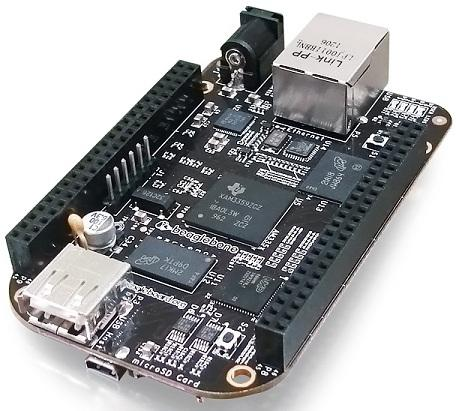
\includegraphics[width=3.5in, height=3in]{images/beaglebone_black.png}
	\caption{BeagleBone Black}
\end{figure}
